\chapter{Introduction} % 10 marzo 2020
\section{Forward contract} \lesson{1}{10/03/2020}
Let's assume that there are two counterparts interested in entering in a contract in the future. This means that at time $t=0$ they want to fix the price $K$ -- called \emph{strike price} -- of whatever (e.g. an asset, an interest rate, an exchange rate, the price of some good) at a future time $T$, called \emph{maturity} of the contract. The two counterparts are called:
\begin{itemize}
    \item \emph{long position}, which at time $T$ has to buy the asset at the price $K$ fixed at $t=0$, regardless the market price;
    \item \emph{short position}, which has to sell the asset at maturity
\end{itemize}
The price of the underlying asset at the current time $t$ is denoted as $S_t$ and it is known/measurable, whereas the price at time $S_T$ is a random variable. This type of contract is called \emph{forward contract}, since we are looking forward in the future. Because it costs nothing to enter into a forward contract, the payoff is also the trader’s total gain or loss from the contract.\\
What can we say about the payoff of the forward contract?
\begin{figure}
    \centering
    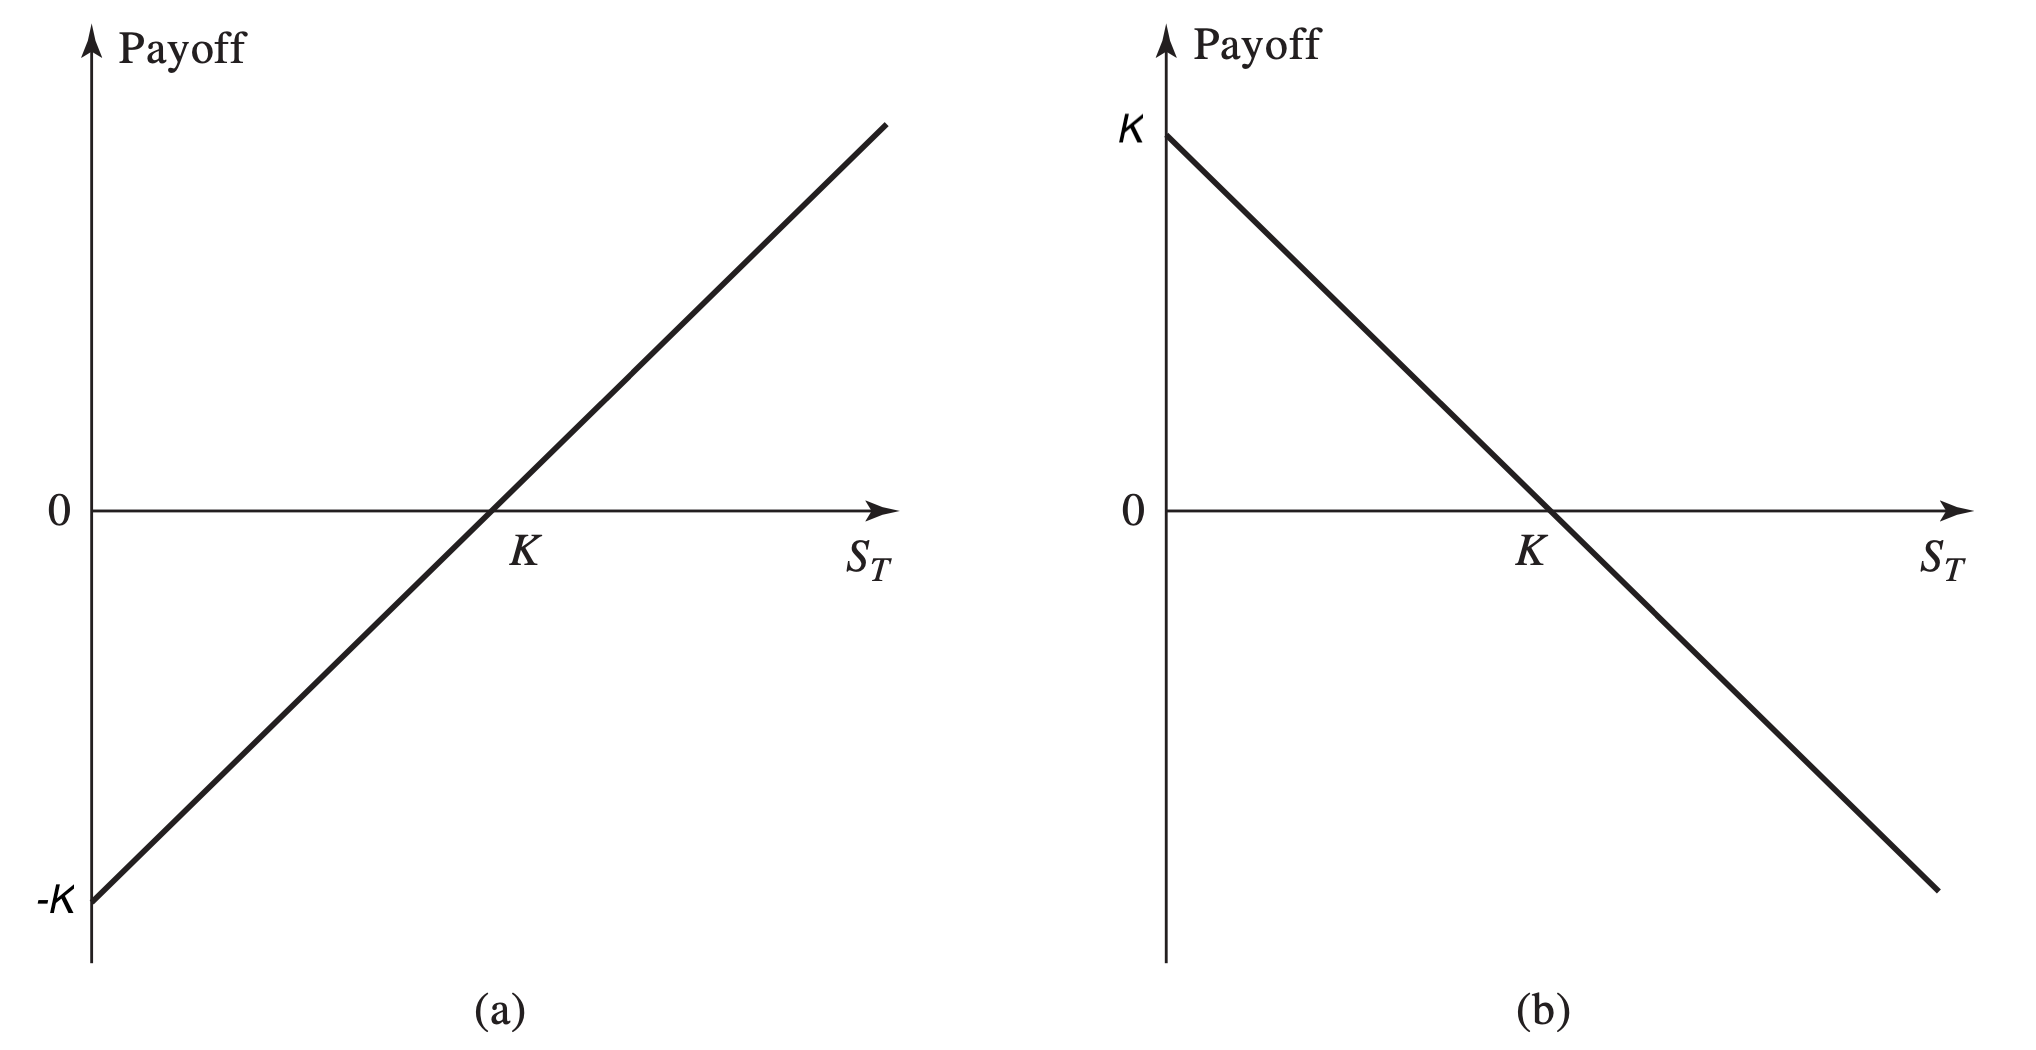
\includegraphics[scale=0.2]{fig/fc_payoff.png}
    \caption{Payoffs from forward contracts: (a) long position, (b) short position.}
    \label{fig:fc_payoff}
\end{figure}
If at time $T$ $S_T>K$ the long position is happy because it has the possibility to buy at $K$ and immediately sell at $S_T$ in the market, getting the payoff $S_T-K>0$. Conversely, if at time $T$ $S_T<K$ the long position is not happy because it buys at $K$ what is worth less in the market. For the short position the situation is symmetric. There are two important considerations:
\begin{enumerate}
    \item For the long position the loss is bounded and the gain is unbounded, whereas for the short position the loss is unbounded and the gain is bounded;
    \item If $K$ changes, for example if $K_2>K_1$, then the long position will not be happy because it wants $K$ to be as small as possible. So, it will not agree to enter in the contract.
\end{enumerate}
So, there is a trade-off between the two counterparts. Our purpose is to find the value of $K$ such that both parts will agree in entering the contract. To do that we have to avoid the presence of an \emph{arbitrage opportunity}, i.e. a possibility of making money for free, without risk (if there is an arbitrage opportunity then fixing a price is meaningless). Quantitatively, an arbitrage opportunity is defined as:
\begin{equation}
    V(t) = \begin{cases}
    0 & t = 0\\
    V_T\ge0 \mbox{ with } \mathbb{P}(V_T\ge0)=1 \mbox{ and } \mathbb{P}(V_T>0)>0 & t=T
    \end{cases}
\end{equation}
In order to avoid arbitrage opportunity we can construct the following portfolio:
\begin{enumerate}
    \item Take a long position in the forward contract. Entering the contract doesn't cost nothing and the payoff is $S_T-K$.
    \item Now we need a contract which gives $-S_T$ at $t=T$. One possibility is selling short: even if we don't have the underlying we borrow it from the broker and we sell it at the current price on the market, promising to re-buy it at time $t=T$ at the price $S_T$.
    \item Now we want to eliminate the $-K$ of step 1, so at $t=T$ we need $+K$ in any case, whatever happens to $S_T$. One possibility is to invest in the riskless market, which basically is the interest rate market\footnote{To be honest, it is not completely riskless, there is the default risk.}. There are two classical notions of interest rate:
    \begin{itemize}
        \item \emph{simple compounding}, which grows linearly in time: $1\to 1+TR$;
        \item \emph{exponential compounding}, which grows exponentially in time: $1\to e^{RT}$.
    \end{itemize}
    So we invest $-Ke^{-RT}$ in the riskless market and at the end we get $-Ke^{-RT}e^{RT}=-K$ changed of sign because at the beginning we spend and at the end we get.
\end{enumerate}
\begin{center}
    \begin{tabular}{lcc}\toprule
        Action & $t=0$ & $t=T$ \\\midrule
        Take a long position in the forward contract &  0 & $S_T-K$ \\
        Sell short & $+S_0$ & $-S_T$ \\
        Invest in the riskless market & $-Ke^{-RT}$ & $+K$ \\ \midrule\midrule
         & $S_0-Ke^{-RT}$ & $0$ \\\bottomrule
    \end{tabular}
\end{center}
In the end the sum at $t=0$ is $S_0-Ke^{-RT}$ and the sum at $t=T$ is zero. Since we want to avoid the presence of no arbitrage opportunity also the sum at $t=0$ has to be zero, otherwise there is an immediate arbitrage opportunity:
\begin{equation}
    S_0-Ke^{-RT} = 0 \quad\Rightarrow\quad K = S_0e^{RT}
\end{equation}
This is the value of $K$ such that both parts will agree in entering the contract.

\section{Options}
Options are derivatives based on the value of underlying securities, such as stocks. An option contract offers the buyer the opportunity to buy or sell -- depending on the type of contract they hold -- the underlying asset. There are two types of option:
\begin{itemize}
    \item a \emph{call} option gives the holder the right to buy the underlying asset by a certain date for a certain price;
    \item a \emph{put option} gives the holder the right to sell the underlying asset by a certain date for a certain price.
\end{itemize}

\subsection{Long call option}
In \emph{long call options} we have the possibility to buy the underlying at time $t=T$ at price $K$ decided at $t=0$. So, at maturity we will buy only if it is convenient.
\begin{figure}[h]
    \centering
    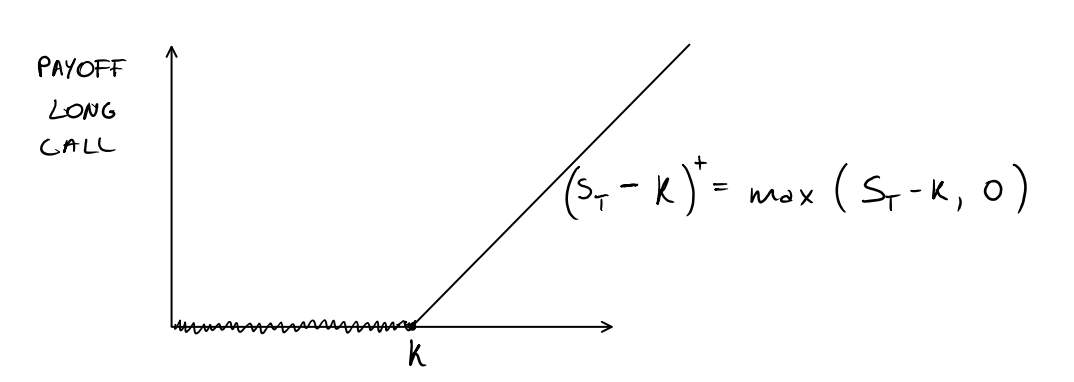
\includegraphics[scale=0.2]{fig/tmp/fig1a}
    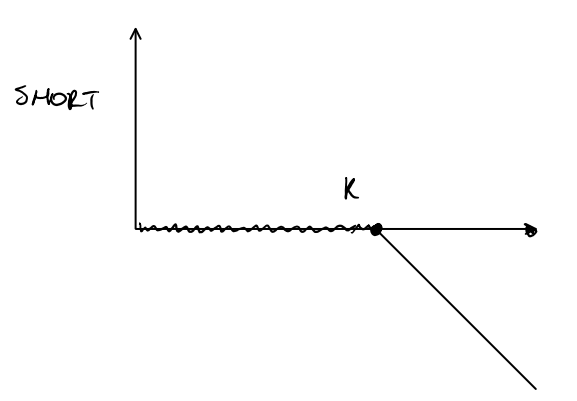
\includegraphics[scale=0.2]{fig/tmp/fig1b}
    \caption{Call option payoffs.}
    \label{fig:figura1}
\end{figure}
\newline Notice that now the payoff is no more linear. If we are in the short position at most we hope to get a zero payoff: nobody will accept this position. This means that the contract will have a price that the long position has to pay to the short position in order to enter the contract. In other words, it is as if the short position sells to the long position the possibility to buy.
\begin{figure}[h]
    \centering
    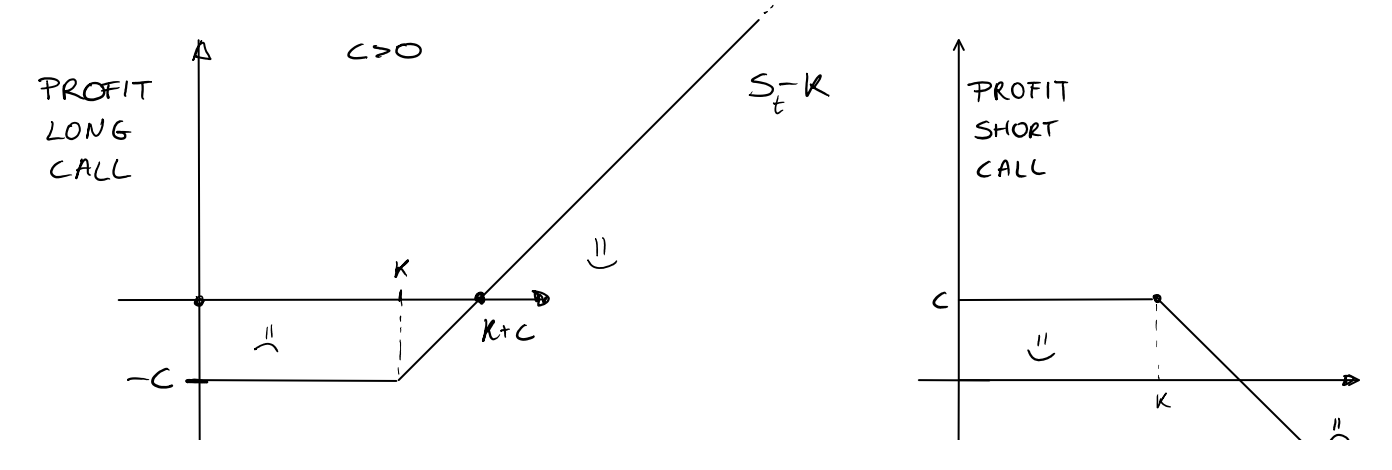
\includegraphics[scale=0.2]{fig/tmp/fig2}
    \caption{Call option profits.}
    \label{fig:figura2}
\end{figure}
\newline If we have different strike prices the corresponding costs will be different. For example, if we have $K_1<K_2$, since the probability to exercise the option corresponding to $K_2$ is smaller than the probability to exercise the option corresponding to $K_1$, then $c_1$ will be larger thank $c_2$:
\begin{equation*}
    K_1 < K_2 \quad\Rightarrow\quad c_1 > c_2
\end{equation*}
\begin{figure}[h]
    \centering
    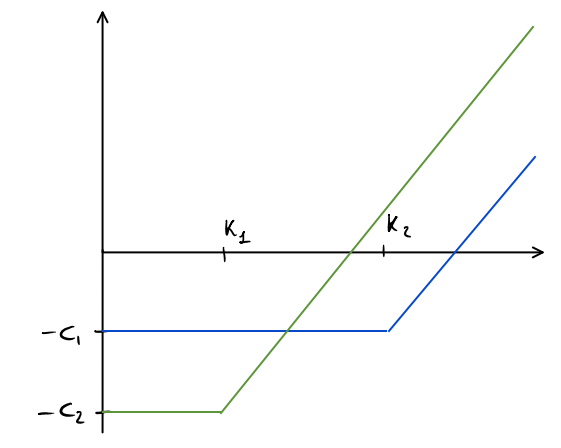
\includegraphics[scale=0.2]{fig/tmp/fig3}
    \caption{Costs for different strike prices.}
    \label{fig:figura3}
\end{figure}

\subsection{Long put option}
In \emph{long put options} we have the possibility to sell the underlying at time $t=T$ at price $K$ decided at $t=0$. So, at maturity we will sell to the counterpart only if it is convenient, i.e. if $S_T<K$\footnote{This is used, for example, by arabian countries which want to avoid that the price of crude oil goes below a certain level.}.
\begin{figure}[h]
    \centering
    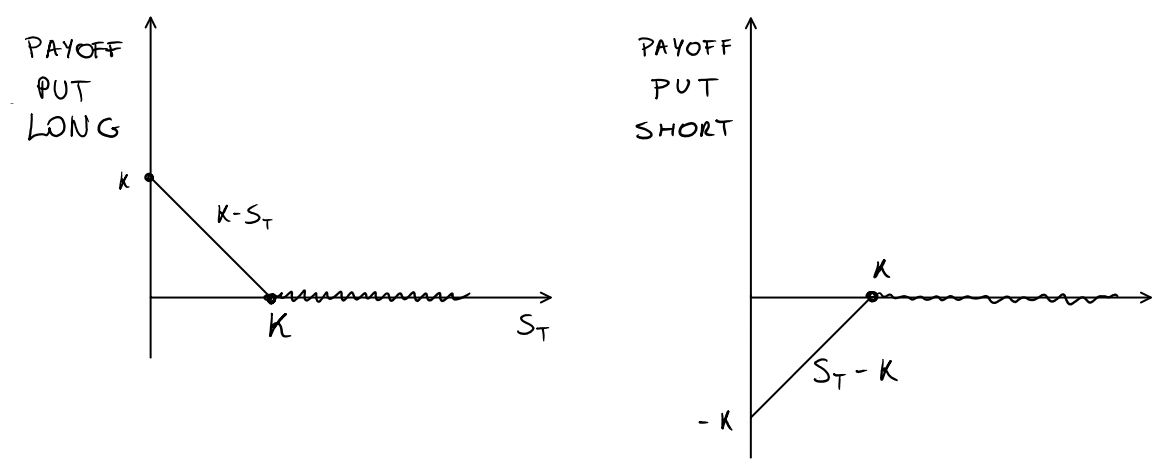
\includegraphics[scale=0.2]{fig/tmp/fig4}
    \caption{Put option payoffs.}
    \label{fig:figura4}
\end{figure}
In this case the short position has the obligation to buy. But there is no convenience in entering such a contract, so again there will be a cost to enter the contract as long position.
\begin{figure}[h]
    \centering
    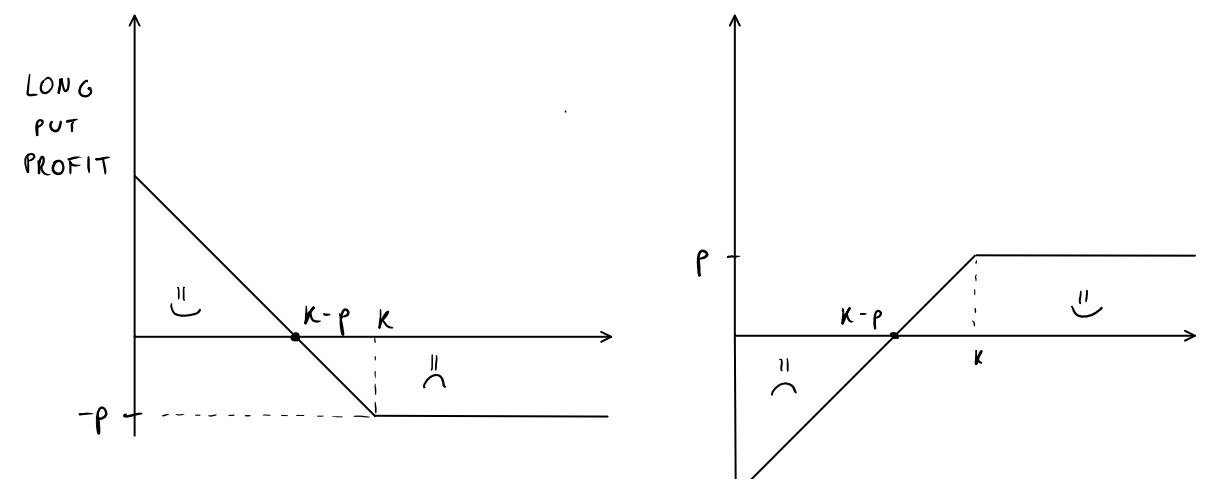
\includegraphics[scale=0.2]{fig/tmp/fig5}
    \caption{Put option profits.}
    \label{fig:figura5}
\end{figure}
If we have different strike prices, for example $K_1<K_2$, since the probability to exercise the option corresponding to $K_2$ is bigger than the probability to exercise the option corresponding to $K_1$, then $c_1$ will be smaller thank $c_2$:
\begin{equation*}
    K_1 < K_2 \quad\Rightarrow\quad c_1 < c_2
\end{equation*}
